\chapter{Background}
This thesis based on several researches of SAS, auto-tuning, evolutionary algorithms and software optimization. To add more understanding of the succeeding chapters this chapter will summarize important aspects and details of approaches and optimization technics are used.  

\section{Multi Quality Auto Tunning (MQuAT)}
Multi-Quality Auto-Tuning (MQuAT) – is approach  to self-adaptive software, , which provides design and operation principles for software systems which automatically provide the best possible utility to the user while producing the least possible cost~\cite{gotz13}.
It is based on design time part which represents a new development method  for  self-optimizing  systems and runtime part which concerns  operation  principles,namely,  novel techniques to runtime self-optimization~\cite{gotz13}.

\subsection{Design principles of MQuAT}
MQuAT presented a new method of developing self-optimized software. In which software is proposed to be constructed from components with specifically defined limits. In addition, components are intended to comprise multiple implementations each providing the same but differing functionality in their non-functional behavior. Therefore, the design principle is the critical factor for runtime optimization because when there is different configuration, optimization can be done and the optimal or almost optimal configuration can be selected. To compare different implementations of software component they need to be specified with their non-functional properties (NFP)~\cite{gotz13}.
To highlight this basic principle a new meta architecture of self optimizing software system was created. It called cool component model~\cite{gotz10}.
A specialty of MQuAT is the application of QoS contracts to cover non-functional implementation behavior as well as the interrelationships of different components between NFPs. Contracts naturally describe the relationship between provisions and requirements.

\subsection{Operation principles of MQuAT}
The core runtime approach proposed in MQuAT is the THE Auto-Tuning Runtime Environment (THEATRE)\cite{gotz10, gotz12}.
The concept of runtime environment  contains three layers: a user, a software and a resource layer. All of them depicted in Figure ~\label{ThreeLayersOfMQuAT}
\todo{pic of three layers o MQuAT}
The user layer invoke features and identify their specifications. The  Global  User  Manager  (GUM)  is  required to manage the mapping between users and software component implementations and to coordinate  the  requests. User requests are minimal software system specifications which have to be met to satisfy the user. The general aim of the runtime system is to help the user as effectively as possible about the purposes of the user~\cite{gotz13}.

Software layer contains all software components and it's implementations. Each component has a Local Quality Manager(LQM) which responsible for the controlling the set of components~\cite{gotz13, ahmad18}. Also, there is a single Global Quality Manager (GQM) which carry out the study and prepare phases of the feedback loop, while the LQM is responsible for the implementation process~\cite{gotz13}.

The resources layer comprises physical (e.g. CPU or RAM) as well as virtual resources(e.g. operating system).
To controlling and monitoring all resources Global Resource Manager(GRM) is presented. Each resource  has its own Local Resource Manager (LRM) which has in-depth knowledge about its resource and the ability to steer the resource by~\cite{gotz13, ahmad18}.

\subsection{MQuAT combine the design time and runtime}
\todo{pic of CombinedMQuAT}
As showed in Figure ~\label{CombinedMQuAT}, in addition to the actual code, the developer is creating the models and quality contracts. The users interact with the system at runtime and prepare their objectives and requests. 
In addition to the running components the runtime system includes a runtime model, representing the current state of the system. The objectives of the user are transformed into objective functions of an optimization program prior to optimization. Depending on the type of optimization technique used, either all users ' objectives are merged into a single objective function or one objective function is extracted per purpose. Such objective functions and the system's runtime model are used by the runtime optimization method to produce formulations of the optimization problem for the respective technique. Finally, the system determines whether the optimal configuration differs from the actual configuration~\cite{gotz13, ahmad18}.

For more details about MQuAT please read refer~\cite{gotz13}. For this thesis,we are discussing a solver of MQuAT problem that is based on MQuAT. Hence, detailed knowledge about MQuAT is not required. 


\section{MQuAT problem}

MQuAT problem was presented in ~\cite{gotz18} and it consist of two problems:

\begin{itemize}
	\item Resource allocation in which the mapping of software component implementation to hardware resource leads to the least cost
	\item Variant selection which provides the best utility by selecting the better software implementations.
\end{itemize} 

To solve this problem was presented new generic metamodel. Both problems are interrelated by user requests specifying minimum requirements on the provided non-functional properties (i.e. minimum utility), while searching for a selection and mapping both to maximize utility and minimize costs. Correctness denotes that only solutions that \textit{do not violate} the users ' minimum requirements are considered \textbf{valid}~\cite{gotz18}.

The problem to be solved is selecting variants of software components and mapping them based on user requests to suitable hardware resources~\cite{gotz18}

The MQuAT problem could be described as a metamodel which consist of:
\begin{itemize}
	\item Hardware metamodel
	\item Software metamodel
	\item The Objective
	\item A Request
\end{itemize}

\subsection{Hardware metamodel}
In Figure~\label{HWmodel} depicted the Hardware metamodel which consist of hierarchically structured resource types and resources as instances of these types. So the hardware model composes static awareness of resources (types) and knowledge of runtime (instances). Certain types of resources can run software, i.e. they are valid targets for software implementation mapping. The container attribute is used to mark such types~\cite{gotz18}.
\todo{pic HWmodel}
In addition, a set of properties further characterize the resource types. Resources specify then specific values for these properties. As an example, the resource type RAM could be defined with a property amount of memory and marked as a container~\cite{gotz18}. 
  
\subsection{Software metamodel}
Figure~\label{SWmodel} depicts Software metamodel and its main element called Component and represents a some functionality.
Each component consist of implementations that provides this functionality, requiring additional components or resources to complete their work. 
\todo{pic SWmodel}

\subsection{Objective}
The Objective specifies how to calculate a solution's objective value, i.e. for which value(s) the problem should be optimized. This selects a property to optimize for, and an objective function to define how to aggregate all values of this property~\cite{gotz18}.

\subsection{Request}
A Request represents a user requirement, which specifies which algorithm should be used to execute parameters and requirements. Requests contain their functional requirements by referring to a target software component, limitations on non-functional requirements (e.g. quality)~\cite{gotz18}.

\subsection{Constrains}
There are some constrains which are grouped in Architectural, Request and Negotiation constraints groups.
\begin{itemize}
	\item Architectural constraints ensure that each request is fulfilled, selecting exactly one implementation per component and deploying no more than one implementation on one resource.
	\item Request constraints ensure components are selected for each request so as to provide the requested non-functional properties.
	\item Negotiation constraints ensure non-functional requirements are met depending on implementation.
\end{itemize}
There are additional constrains due to problem generation:
\begin{itemize}
	\item structures for the software and hardware components are fixed to ensure comparability,
	\item computeNode that represents a regular computer hardware consist of one or more CPUs, RAM memory, disk, and a networking interface,
	\item software model has a simple tree structure,
	\item  fixed branching factor of two~\cite{gotz18}.
\end{itemize}


\todo{Should I add parameters that describes a problem(software variants, number of requests and so on)?)}
\section{The solution of the MQuAT problem}
The solution is computed by the MQuAT solver. There are many solvers but we will talk only about one of them a bit latter.
The solution could be represented as a tree structure. An example of solution shown in Figure~\label{SolutionModel}
\todo{pic SolutionModel}
It contains a list of assignments. Each assignment select one implementation of required component and map it to the resources~\cite{gotz18}.
A solution is valid if for each user request
\begin{enumerate}
	\item an implementation is deployed for the target component,
	\item for each component required an implementation is deployed,
	\item all necessary (non-functional) property clauses (including request constraints) are met,
	\item at most one implementation for each resource is deployed.
\end{enumerate}
If it is valid and no other solution has a better objective value, then a solution is optimal~\cite{gotz18}.
     
\section{Genetic algorithm}
Evolutionary algorithms is a subset of evolutionary computation and belongs to set of modern heuristics based search method.~\cite{vikhar16}
Appeared as a result of the influence the biological evolution on computer scientists. This domain contains different types.
There are
\begin{itemize}
	\item Genetic algorithm 
	\item Genetic programming
	\item Evolutionary programming
	\item Evolution strategy
\end{itemize}

Genetic algorithm (GA) is the most popular type of EA.

\begin{figure}
	\centering
	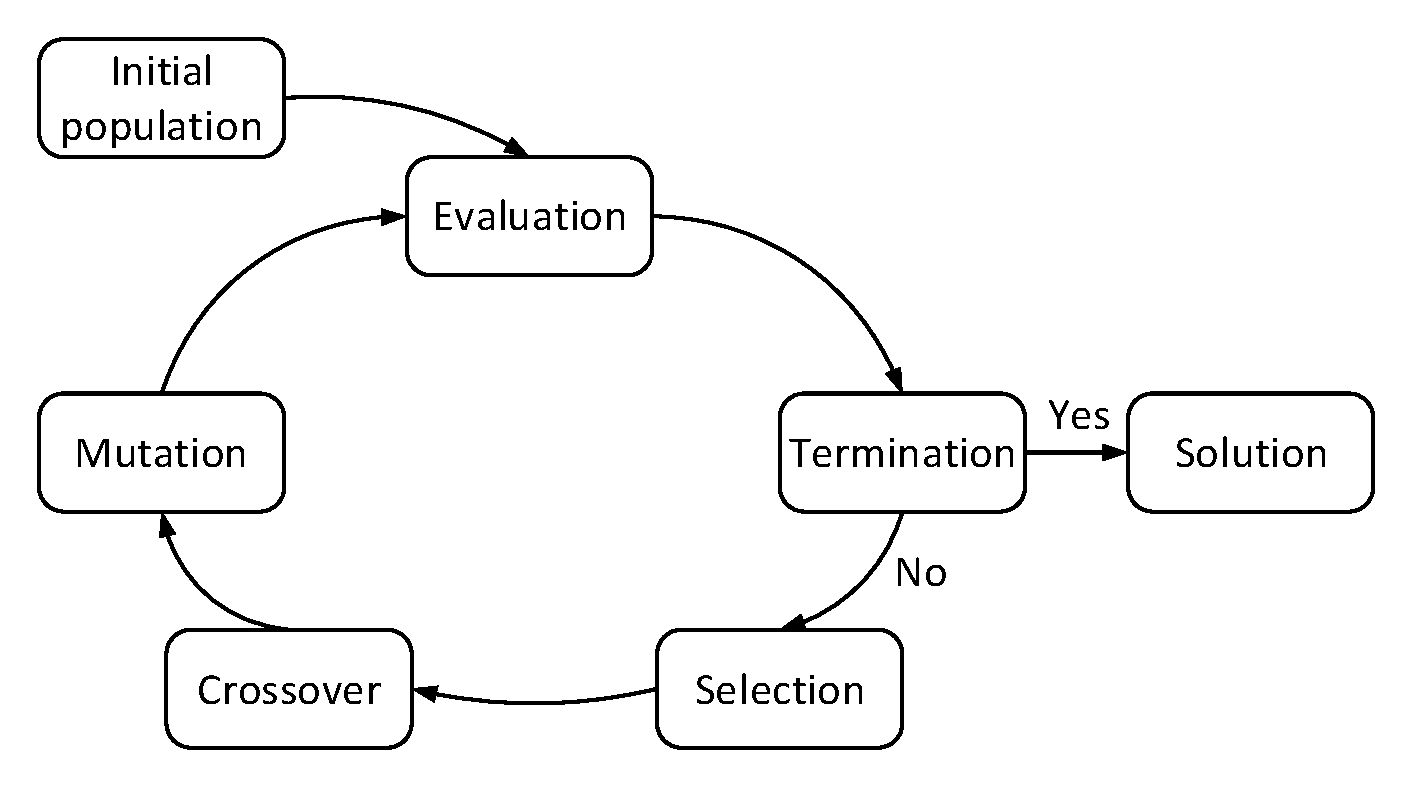
\includegraphics{images/GeneticLoop}
	\caption{Main loop of the genetic algorithm}\label{fig:GeneticLoop}
\end{figure}
Main principle of GA looks like a loop with several steps.
First step is creation of initial population - a set of randomly created individuals each of them represent one solution. 
Second step is Evaluation. Calculate fitness or objective function of current population.
If solution is founded and all requirements for the termination are fulfilled then we will get the final solution. Otherwise, select best candidates to create new generation.
In step 4 using recombination and mutation on selected candidates GA creates new generation of population. And after that evaluate it.

GA based on different components and operators.
\subsection{Selector}
Selector is one of the most important components of GA. It selects \textit{mu} number of individuals from the population. The motivation of this operation come from Charles Darwin's theory of natural selection. He says that the most fitted or adapted individuals have a better chance to get better offspring.

There are many different selection algorithms
\begin{itemize}
	\item NSGA2 (Non-dominated sorting based genetic algorithm)
	\item SPEA2 (Strength Pareto Evolutionary Algorithm)
	\item NSGA3\todo{litref}
	\item SPEA3\todo{litref}
	\item PDE \todo{litref}
\end{itemize}
In this thesis we will focus on selection algorithm only as a parameter of genetic algorithm and will use NSGA2 and SPEA2. 
\todo{Do I need to describe how works NSGA2 and SPEA2?}
\subsection{crossover}
Crossover is an operator of genetic algorithm that allows recombination of two individuals by swapping some genes between them.
In general, crossover has a several parameters such as
\begin{itemize}
	\item Crossover rate - parameter that describes the probability of two chromosomes to exchange their genes.
	\item Crossover point - the point in which the exchange could be done.
\end{itemize}

The principle of the crossover is next.
Firstly, select the crossover point. For example, chromosome could be described as a vector of bits, then the crossover point will be the start index of bits which will be replaced from another chromosome.
Secondly, swap genes between chromosomes.

\todo{fig}

\subsection{mutation}

Mutation is an operator of genetic algorithm that change single gene in a chromosome. As a crossover operator, mutation has parameters:

\begin{itemize}
	\item Mutation rate - parameter that describes the probability mutation.
\end{itemize}

To perform mutation on chromosome need to do:
\begin{enumerate}
	\item Randomly select gene which will mutate
	\item Change selected gene to another.
\end{enumerate}

On the \todo{fig} presented simple mutation on chromosome that described as a vector of bits.

\todo{fig}

\section{Genetic solver}
To solve MQuAT problem using genetic algorithm genetic solver was developed by Jamal Ahmad in ~\cite{ahmad18}. And further improved by Johannes Mey.

This solver is based on Opt4J\todo{link to website} framework. It's an open-source framework that gives the opportunity to implement genetic algorithm for custom optimization problem by specifying several modules and classes.

To solve custom problem using genetic algorithm user need to create several things:
\begin{enumerate}
	\item Creator
	\item Decoder
	\item Evaluator
\end{enumerate}
Also, if your genotype can't be described as vector, then you firstly need to implement:
\begin{enumerate}
	\item Genotype
	\item Crossover operator
	\item Mutation operator
\end{enumerate}

\subsection{Tree Shape Genotype}
Because of problem model of MQuAT in genetic solver was created Tree Shape Genotype~\cite{ahmad18}.

\todo{will add more}.
 
\subsection{Crossover operator}
This operator perform crossover between two Tree Shaped Genotypes. 

\todo{fig}



\subsection{Mutation operator}
This operator perform crossover between two Tree Shaped Genotypes. 

\todo{fig}

\subsection{Creator}
\label{subsec:Creator}
Genetic algorithm uses creator to create random genotypes for initial population.
In genetic solver Creator create the genotype by creating random solution model and transform it to Three Shape Genotype structure.

\todo{fig}

\subsection{Decoder}

Decoder decode genotype into phenotype.
Phenotype is a solution that could be evaluated.
In genetic solver decoder transform genotype to Solution Model of MQuAT.

\todo{fig}

\subsection{Evaluator}

Evaluator calculate objective functions of the solution. 
In genetic solver the evaluator calculates two objectives:

\begin{enumerate}
	\item Validity errors - number of violated contracts
	\item Energy value - energy consumption
\end{enumerate}

\section{Parameter Tuning Strategies for GA}
information from literature!\todo{will add more in next draft}

\section{BRISE}
BRISE is a software product line (SPL) for parameter tuning.
BRISE has a distributed structure and consist of three components.
\begin{itemize}
	\item Main Node
	\item Worker Service
	\item Worker
\end{itemize}
All this components works as a docker containers and communicate between themselves using queens. 
\todo{fig of architecture}

\subsection{Main node}
\todo{fig of main node}
Main Node is a core component of the framework, it is responsible for the whole flow of the application except the measurement process.~\cite{pukhkaiev19} 

\subsection{Worker Service}
\todo{fig of main node}
Main node - is a main component and it's 

\subsection{Worker}
\todo{fig of main node}
Worker is a lightweight component, containing only the logic of the algorithm to be tuned (or its wrapper), which should be specified by the user. It gets a parameter combination to be tested as an input and outputs the quality metric to be later evaluated in the Main Node. 








